\chapter{Implementacja}

\section{Dane wejściowe}
Krok przemiany danych wejściowych do wykorzystania w module został podzielony na dwa osobne etapy. Jeden z tych etapów, nazywany krokiem interpretacji różni się w zależności od źródła skąd pochodzą dane. W zależności od tego, czy system korzysta z danych historycznych w procesie uczenia, czy korzysta z danych aktualnych w celu predykcji inaczej przechodzą proces interpretacji. Drugim etapem jest etap transformacji i wygląda on tak samo dla każdego źródła niezależnie od typu.

\subsection{Interpretacja historyczna}
W przypadku źródła danych historycznych, system musi rozpoznawać epizody działań domowników w celu ich nauki. W tym celu, aby wygenerować zbiór danych uczących, przegląda się posortowaną listę wydarzeń w czasie, celem określenia epizodów akcji. Począwszy od pierwszego wydarzenia w dostępnej dla systemu historii, przegląda się ją w poszukiwaniu ciągu akcji o łącznym czasie nie większym niż pewien z góry określony parametr nazwany \verb+EPISODE_DELTA+ od momentu wystąpienia pierwszej akcji w epizodzie. Ta wartość została wprowadzona w celu sprawdzenia czy zmiana stanu w epizodzie się nie przedawniła. W przypadku gdy jedno urządzenie zmienia swój stan kilkukrotnie w przeciągu jednego epizodu, brana jest tylko pod uwagę policzona zmiana i stan względem poprzedniego, przed liczonym epizodem. W tabeli (\ref{tab:znaleziony_epizod}) został zaznaczony znaleziony dla przykładowej historii epizod. Kolorem został zaznaczony znaleziony przez algorytm epizod akcji. 

Warto zauważyć, że wybrana długość tego parametru będzie mocno wpływała na liczność i wielkość epizodów. Wybranie zbyt krótkiego czasu epizodu będzie rozdzielać powiązane ze sobą czynności ale będzie rozróżniała zmiany stanu tego samego urządzenia w czasie, a wybranie zbyt długiego czasu będzie łączyło kilka niezależnych akcji ze sobą, możliwie je ze sobą niwelując. Sprawia to, że wybranie optymalnej długości epizodu jest bardzo ważne aby system mógł dostosować się do użytkownika.

\begin{table}
    \centering\caption{Tabela przedstawiająca działanie algorytmu szukania epizodów. \label{tab:znaleziony_epizod}}
    \begin{tabular}{|l|l|l|}
        \hline
        Urządzenie              & Stan       & Czas     \dnl
        \dots                   & \dots      & \dots    \nl
        \verb+światło kuchnia+  & \verb+on+  & 16:52:48 \nl 
        \rowcolor{lightgray}
        \verb+światło kuchnia+  & \verb+off+ & 17:32:12 \nl 
        \rowcolor{lightgray}
        \verb+klimatyzacja+     & \verb+17+  & 17:33:00 \nl 
        \rowcolor{lightgray}
        \verb+światło salon+    & \verb+on+  & 17:33:10 \nl
        \rowcolor{lightgray}
        \verb+telewizor salon+  & \verb+on+  & 17:33:15 \nl
        \verb+światło balkon+   & \verb+on+  & 19:32:42 \nl
        \dots                   & \dots      & \dots    \nl
    \end{tabular}
\end{table}

Do określenia działania, dla każdego innego typu urządzeń z osobna, skorzystano z abstrakcyjnej klasy \verb+DeviceHistoryGeneric+, opisujących strukturę funkcji jakie powinna dana klasa implementować w celu poprawnego działania. Abstrakcyjna funkcja na podstawie stanu urządzenia w momencie $t$, stanu urządzenia w momencie $k$ oraz czasu do którego dany epizod powinien się skończyć, zwraca w postaci rzeczywistej liczby, stan oraz przejście stanu dla danego epizodu w czasie. Pseudokod takiej funkcji został zawarty w listingu (\ref{listing:pseudo_get_past_state}). Warto zauważyć, że gdy nie ma poprzedniego stanu, tj. historia nie sięga na tyle wstecz, to kod musi obsługiwać wykrywanie obu wartości. W przypadku interpretacji prostych urządzeń, nie jest to problemem, ponieważ jesteśmy w stanie wydedukować przejście stanu i aktualny stan na podstawie informacji pochodzącej z systemu, tak w przypadku gdy tej możliwości nie ma, pojedynczy błędny wynik powinien być zdecydowaną mniejszością po interpretacji reszty historii.

% todo: zapytać o ten pseudokod
\begin{listing}
\begin{minted}[mathescape]{python}
def get_past_state(aktualny, poprzedni, do_momentu):
    wartość_stanu = 1.0 jeśli aktualny = "on" wpw 0.0
    wartość_przejścia = 0.0
    # Czy mamy historię na temat poprzedniego?
    jeśli poprzedni nie istnieje:
        # zakładamy, że zmiana stanu odbyła się dawno w historii
        return wartość_stanu, wartość_przejścia
    
    # Czy zmiana się nie przedawniła?
    jeśli poprzedni.czas_zmiany < do_momentu:
        wartość_przejścia = 1.0 jeśli aktualny = "on" wpw -1.0

    return wartość_stanu, wartość_przejścia
\end{minted}
\caption{Pseudokod funkcji interpretującej stany ze źródła historycznego dla typu urządzenia przełącznika astabilnego on/off.} \label{listing:pseudo_get_past_state}
\end{listing}

% Zebrane w ten sposób dane, zbierane są jako listy słowników języka Python w celu łatwiejszego 

\subsection{Interpretacja bieżąca} \label{subsec:interpretacja}
Bieżąca interpretacja akcji użytkownika wygląda bardzo podobnie do analizy historycznej. Informacja o bieżącym stanie całego systemu przechowywana jest przez moduł w pamięci. Podczas pracy systemu, mamy pewność, że system AppDaemon zgłosi zmianę stanu tylko jednego urządzenia za każdym uruchomieniem naszej asynchronicznej funkcji. Wiemy zatem, że musimy tylko obsłużyć zmianę stanu jednego urządzenia i zapisać jego stan do pamięci. Informacja o tym, jakie urządzenie zmieniło się do jakiego stanu będzie potrzebna w procesie predykcji, które będzie opisane w późniejszym etapie. Korzystając z tej samej klasy dla typu urządzenia co w przypadku interpretacji historycznej w podobny sposób określamy stan i przejście stanu urządzenia. W tym wypadku ze względu na pewność, że dane urządzenie zmieniło swój stan dokładnie w momencie uruchomienia danej funkcji, obliczanie stanu i przejścia jest zdecydowanie prostsze ponieważ, nie trzeba rozważać przedawnienia się zmiany.

\subsection{Transformacja}
Po prawidłowej ekstrakcji zmian stanu, przed przekazaniem ich do sieci neuronowych dane są dodatkowo przekształcane. W przypadku prostych urządzeń typu przełączniki astabilne, ten proces nie wprowadza do danych żadnej zmiany. W przypadku bardziej skomplikowanych typów danych, takich jak zmienne temporalne wskazujące na np. dzień tygodnia, czy porę dnia, przeprowadzane są pewne dodatkowe operacje rozkładające jedną konkretną informację na kilka różnych wartości, które lepiej będzie sieciom neuronowym powiązać ze akcjami. W celu możliwości wprowadzenia rozszerzalności tutaj ponownie wykorzystano podejście obiektowe i skorzystano z klasy abstrakcyjnej. Zaproponowana klasa abstrakcyjna \verb+Convertable+ opisuje dwie funkcje, które dany konwerter danych musi zaimplementować. Jedna z nich opisuje przejście danych do wersji akceptowalnej przez sieci neuronowe, druga tłumaczy dane wygenerowane przez sieć neuronową do formy obsługiwanej przez resztę systemu. Jednym specjalnym przypadkiem takiego konwertowania danych gdzie potrzebna jest zaimplementowana jedna z obu funkcji, jest przekazywanie zmiennych temporalnych do sieci.

W celu przekazania do sieci jak największej ilości rzeczywiście użytecznych informacji o porze dnia, tak aby była ona w stanie w swojej strukturze zapisać nawyki użytkownika, informacja o czasie jest podzielona. Podział jednej zmiennej czasowej odbywa się poprzez podzielenie jej na 24 różne informacje, gdzie każda z nich wskazuje na pewną wartość zależną od odległości indeksu danej zmiennej od godziny wydarzenia epizodu. Dokładniej, jest to wartość funkcji Gaussa dla wartości zależnej od indeksu, z parametrem $\mu$ ustawionym na moment w ciągu dnia podczas którego wydarzył się ten epizod.

Ważnym parametrem w przypadku funkcji Gaussa poza parametrem $\mu$, jest parametr opisujący szerokość dzwona. W zastosowaniach statystycznych nazywany odchyleniem standardowym $\sigma$. W przypadku takiego zastosowania obliczania wartości funkcji na podstawie czasu, szerokość mówi nam o tym, jak bardzo akcje występujące o konkretnej porze w ciągu dnia mogą być proponowane o innych podobnych godzinach. Ustawienie tego parametru zbyt szeroko, spowoduje że system będzie rozpoznawał wykonywanie konkretnych akcji o bardzo szczegółowych godzinach w ciągu dnia, ustawienie tego za szeroko, będzie proponowało wykonywanie akcji nieadekwatnych do konkretnej pory dnia. Na obrazie (\ref{fig:time_param}) znajduje się przykładowy zarys wartości funkcji dla kilku konkretnych pór dnia, razem z zaznaczonymi dokładnymi przebiegami krzywizny dzwonowej. Każda z zaznaczonych godzin posiada inny parametr $\sigma$ w celu pokazania wpływu tego parametru na policzone wartości.

\begin{figure}
    \centering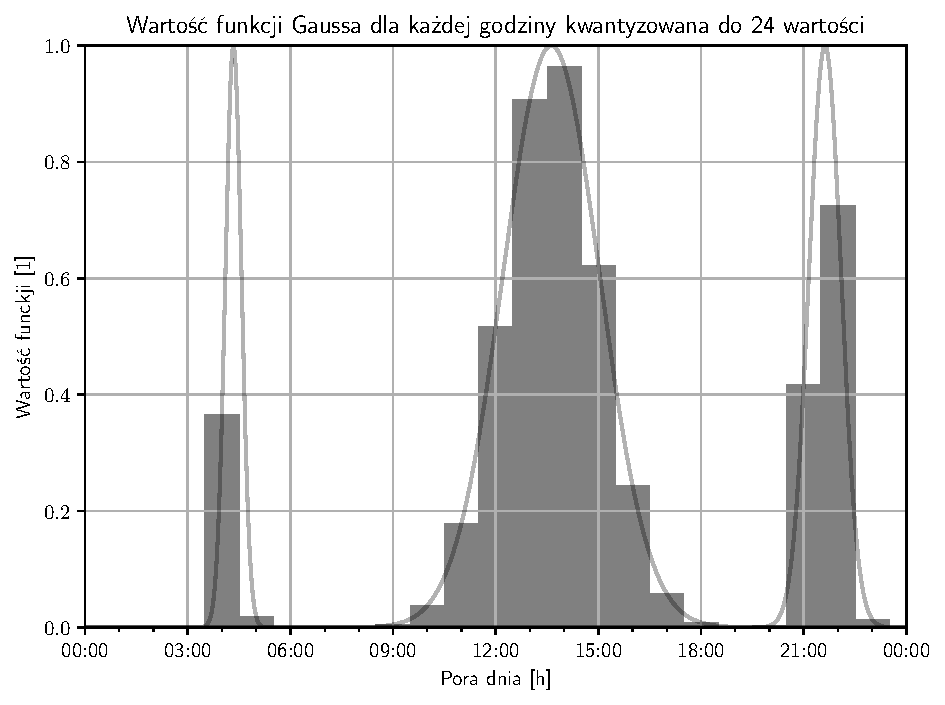
\includegraphics[width=1.00\textwidth]{img/time_param.pdf}
    \caption{Policzone wartości funkcji Gaussa wskazującej czas dla godziny 4:20:02, 13:37:21, 21:37:21.} \label{fig:time_param}
\end{figure}


\section{Sieci neuronowe}
Ze względu na wymóg osobnego przetwarzania wielu źródeł różnego typu w systemie, gdzie część z nich może kolejno zostać jeszcze podzielona na dalsze drobniejsze informacje, całość systemu została umieszczona w obiekt będący menedżerem. Głównym zadaniem menedżera jest agregowanie do jednego obiektu wielu konwerterów i agentów. Agent w tym systemie, to obiekt z pewnymi z góry określonymi funkcjami opakowujący modele matematyczne dostarczone przez bibliotekę Tensorflow wykorzystywany do schowania za warstwą abstrakcji, detali implementacji \cite{book:programming_abstraction}, \cite{book:czysty_kod}. Takie wykorzystania menedżerów i obiektów agregujących przydaje się w przypadku tworzenia systemów dynamicznych polegających na wczytywaniu i zapisywaniu obiektów do pamięci stałej. W przypadku tego modułu samouczącego, daje to osobie rozszerzającej, możliwości wykorzystania innych struktur niż wcześniej określono (\ref{tab:neural_network}) lub nawet wykorzystanie kompletnie innych metod predykcji w celu osiągnięcia danego celu.

\subsection{Dynamiczne tworzenie}
Jedną bardzo wygodną możliwością udostępnianą przez bibliotekę Tensorflow dla modeli sieci neuronowych są nazwane wyjścia oraz wejścia dla sieci. Pozwala to na dynamiczne tworzenie i eksploatację modeli bez żadnego bardzo skomplikowanego systemu przetwarzającego nazwę wejść na globalną pozycję w macierzy wejściowej. System w celu stworzenia modelu sieci neuronowej wykorzystuje obiekt \verb+Model+ udostępniany przez bibliotekę wykonawczą Tensorflow -- Keras. Do stworzenia modelu sieci neuronowej, korzystamy z informacji o nazwach wejść oraz nazwach wyjść. System podczas tworzenia nowej sieci, tworzy listę warstw typu \verb+Input+ i każdej z nich przypisuje nazwę kolejnego wejścia do sieci, następnie każda z tych warstw, o kształcie \verb+(wielkość próbki, 1)+, jest do siebie dodawana wzdłuż drugiego wymiaru za pomocą warstwy typu \verb+Concatenate+. Powstała warstwa ma kształt \verb+(wielkość próbki, ilość wejść)+. W tym momencie kolejne warstwy dodaje się tak samo jak w przypadku zwykłego modelu funkcyjnego biblioteki Tensorflow i następuje zgodnie z listą warstw podaną we wcześniejszym rozdziale (\ref{tab:neural_network}). Ostatnia warstwa, ta wyjściowa, tak jak w przypadku warstw wejściowych generowana jest z listy nazw wyjść. Dynamiczne tworzenie wyjść, razem z modelem modularnej transformacji, opisanej wcześniej, daje bardzo potężne narzędzie do sterowania domem.

\subsection{Serializowanie i deserializowanie}
Zapis oraz import danych w systemach komputerowych z formy istniejącej w pamięci do formatu, którą można zapisać na dysk jest bardzo dużym zagadnieniem samym w sobie. W przypadku języka Python jest bardzo dużo możliwości godnych tego zadania. Istnieje wbudowana biblioteka taka jak Pickle, która zapisuje wprost bit po bicie zawartość pamięci programu do pliku na dysku, ale zapisuje bardzo dużo redundantnych informacji nad którymi nie mamy kontroli. Istnieją rozwiązania które są czytelne dla ludzi, ale osiągają mniejszą efektywność zapisu danych, takie jak XML \cite{book:xml_handbook} czy JSON \cite{book:json_for_begginers}. 

W wypadku zapisu i odczytu modeli matematycznych potrzebna jest obsługa trzech różnych informacji, które zostały wymienione wcześniej (\ref{subsec:nn}). Opis logicznej struktury sieci, składa się z informacji o każdej z warstw. Każda z warstw zawiera informacje o jej wielkości, typie, rodzaju aktywacji, nazwach oraz informacji z jakimi warstwami sąsiaduje. Dostarczana przez Tensorflow metoda dla obiektu modelu zwraca wszystkie te informacje w postaci słownika, zawierającego tekst, listy oraz kolejne warstwy słowników. Klasa odpowiedzialna za model implementuje konstruktor \cite{book:czysty_kod}, który korzystając z informacji zawartych w opisanym słowniku odtwarza dokładną strukturę modelu. Sytuacja wygląda bardzo podobnie dla wag w modelu. Każda warstwa udostępnia funkcję zwracającą listę wszystkich ważnych dla danego typu warstwy parametrów, a druga w obiekcie modelu, przyjmuje listę tych parametrów w celu odtworzenia wag.

W celu implementacji zapisywania i odczytu danych z dysku skorzystano z wbudowanej w Python biblioteki obsługującej pliki \verb+.zip+ oraz z metody serializacji JSON. Do obsługi procesu zapisu i odczytu stworzono klasę \verb+ModelSerializer+, implementującą metody potrzebne do skorzystania z danego obiektu jako menedżera kontekstu języka Python \cite{book:learning_python}. Taki sposób implementacji zapewni, że wszystkie wymagane operacje na pliku i buforach w pamięci zostaną wykonane bez ingerencji użytkownika, co pozwoli na uniknięcie błędów. Stworzony obiekt dostarcza dwie główne metody. Jedna z nich służąca do odczytu i odtworzenia całej struktury menedżerów do takiej wykorzystanej przez moduł oraz drugiej wykorzystywanej do zapisu całego menedżera do pamięci stałej, które działają analogicznie w odwrotnym kierunku.

Pewną emergentną zaletą takiego połączenia serializowania za pomocą JSON wewnątrz kompresowalnego archiwum plików jest zmniejszenie miejsca które zajmują wszystkie modele na dysku, o nawet 57\%. Opis wytworzonego w ten sposób archiwum znajduje się w listingu (\ref{listing:zipinfo}).

\begin{listing}
\begin{minted}{text}
Zip file size: 698977 bytes, number of entries: 19
?rw-------  2.0 unx     8626 b- 23-Nov-22 10:47 kuchnia/declaration.json
?rw-------  2.0 unx   264887 b- 23-Nov-22 10:47 kuchnia/weights.json
?rw-------  2.0 unx       59 b- 23-Nov-22 10:47 kuchnia/meta/info.json
?rw-------  2.0 unx     8640 b- 23-Nov-22 10:47 ekspres/declaration.json
?rw-------  2.0 unx   265319 b- 23-Nov-22 10:47 ekspres/weights.json
?rw-------  2.0 unx       59 b- 23-Nov-22 10:47 ekspres/meta/info.json
?rw-------  2.0 unx     8646 b- 23-Nov-22 10:47 salon/declaration.json
?rw-------  2.0 unx   265341 b- 23-Nov-22 10:47 salon/weights.json
?rw-------  2.0 unx       59 b- 23-Nov-22 10:47 salon/meta/info.json
?rw-------  2.0 unx     8648 b- 23-Nov-22 10:47 telewizor/declaration.json
?rw-------  2.0 unx   265556 b- 23-Nov-22 10:47 telewizor/weights.json
?rw-------  2.0 unx       59 b- 23-Nov-22 10:47 telewizor/meta/info.json
?rw-------  2.0 unx     8656 b- 23-Nov-22 10:47 balkon/declaration.json
?rw-------  2.0 unx   265197 b- 23-Nov-22 10:47 balkon/weights.json
?rw-------  2.0 unx       59 b- 23-Nov-22 10:47 balkon/meta/info.json
?rw-------  2.0 unx     8658 b- 23-Nov-22 10:47 sypialnia/declaration.json
?rw-------  2.0 unx   265469 b- 23-Nov-22 10:47 sypialnia/weights.json
?rw-------  2.0 unx       59 b- 23-Nov-22 10:47 sypialnia/meta/info.json
?rw-------  2.0 unx      273 b- 23-Nov-22 10:47 info.json
19 files, 1644270 bytes uncompressed, 696557 bytes compressed:  57.6%
\end{minted}
\caption{Listowanie plików wewnątrz archiwum zawierajacego przykładowe modele sieci pochodzące z programu zipinfo.} \label{listing:zipinfo}
\end{listing}

\section{Sterowanie systemem}
Gdy dane o stanie z dołączonymi innymi informacjami temporalnymi przejdą przez cały system i jest zwracana predykcja, system musi podjąć decyzję czy to co aktualnie użytkownik tych urządzeń wykonuje, jest zgodne z tym co system przewiduje. Jak wcześniej zostało opisane, system stara się przewidzieć następną zmianę stanu na podstawie przekazanych do modelu wartości o aktualnym stanie. Aby system był jak najbardziej wygodny dla użytkownika, zdecydowano na dopełnianie akcji użytkownika zamiast wykonywanie zadań autonomicznie. Sprawia to, że proces wyboru kiedy system powinien dokończyć daną akcję staje się bardzo skomplikowany.

W celu wykonywania tylko tych akcji, które są w danym momencie zgodne z zamiarem użytkownika porównywane są predykcje systemu z aktualną zmianą, na którą moduł reaguje. Dane wejściowe policzone z interpretacji bieżącej (\ref{subsec:interpretacja}) porównywane są z tym co przewiduje system. Jeśli zamiar użytkownika jest wspólny z tym co system chce wykonać, system podejmuje decyzję o dokończeniu przewidzianego epizodu akcji. Porównanie zamiaru jest trywialne i porównuje obliczone aktualne przejście stanu dla danego urządzenia oraz to, które powstało z predykcji. Korzystając z informacji o aktualnym stanie, przewidzianej zmiany, generowane są zapytania do systemu mające na celu sprowadzenie systemu do nowego stanu.

\section{Formatowanie danych uczących}
Uczenie sieci neuronowych z danych pochodzących z historii HomeAssistant często samo w sobie jest niewystarczające. Sieci mimo tego, że uczone są na dużej ilości danych temporalnych poza samymi stanami systemu, nie są w stanie nauczyć się konkretnych epizodów. W tym celu, zaproponowano generowanie dodatkowych danych uczących na podstawie wygenerowanych informacji o przejściach, aby poprawić celność systemu.

Algorytm generowania danych tworzy dodatkowe informacje wejściowe zawierające brak zmiany stanu dla konkretnego stanu systemu o innej porze dnia niż wtedy kiedy dany epizod jest wykonywany. W tym celu funkcja tworzy dwa słowniki, jeden dla którego wartościami są listy zawierające czas pewnego wydarzenia, druga dla której wartości to zbiory zmiany stanów. W obu tych słownikach, kluczami są stany dla którego rozpatrywany jest czas czy zmiana. Dalej, dla każdego czasu kiedy dane zdarzenie sie wydarzyło, czyli dla elementow w pierwszym z obu słowników, generowany jest estymator jądrowy danego wydarzenia. W tym celu wykorzystano sumę rozkładów normalnych. Następnie wygenerowany estymator jest odwracany i progowany. Wszystkie wartości powyżej lub poniżej pewnego przedziału są spłaszczane do wartości brzegowych, a następnie przekształcane i skalowane tak, aby suma pola pod wykresem wynosiła 1, a najmniejszą wartością było 0. Proces ten został zobrazowany na obrazie (\ref{fig:transform}). Korzystając z tak wygenerowanego estymatora znormalizowanego i funkcji losującej wartość z przedziału pod warunkiem macierzy prawdopodobieństw, dostarczonej przez numpy, generowany jest zestaw zerowych przejść z czasem pochodzącym z tego rozkładu, a następnie dołączany do listy danych do uczenia. Ten proces ma na celu stworzenie listy dodatkowych danych bez żadnej zmiany dla konkretnego stanu o innej porze w ciągu dnia, tak aby sieci neuronowe powiązały konkretny stan w ciągu dnia z konkretną porą dla danej odpowiedzi. Tak stworzona lista dla konkretnych stanów jest bardzo rzadka -- posiada same zera w przejściach stanów -- co może negatywnie wpłynąć na wynik uczenia sieci neuronowych. W tym celu, aby zrównoważyć stosunek ilości pustych akcji do tych rzeczywistych, do listy danych uczących dodawane są kolejne dane. Dane te losowane są z drugiego słownika dla konkretnie obsługiwanego stanu systemu i dodawane do danych uczących, czyli dopisywane są kopie danego rzeczywistego wydarzenia.

\begin{figure}
    \centering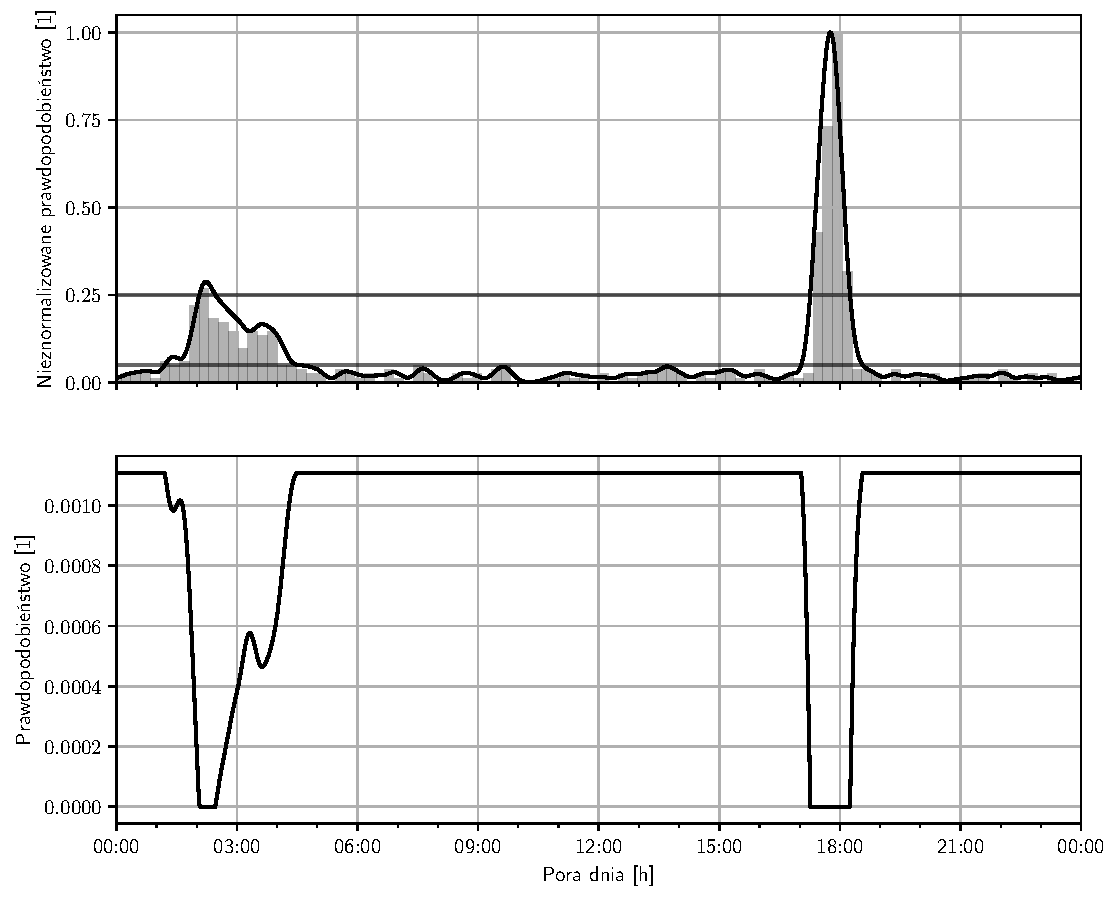
\includegraphics[width=1.00\textwidth]{img/transformation.pdf}
    \caption{Wizualizacja wygenerowanego estymatora jądrowego bez progowania oraz przebieg gotowej funkcja gęstości prawdopodobieństwa.} \label{fig:transform}
\end{figure}


% \section{Struktura wewnątrz Docker'a}

% wykorzystanie warstw abstrakcji jest lepsze ...